% Author: Alfredo Sánchez Alberca (asalber@ceu.es}
% !TEX program = xelatex
\documentclass[aspectratio=149,10pt,t]{beamer}
%-------------------------------------------------------------------------------
% GENERAL PACKAGES
%-------------------------------------------------------------------------------
% Language
\usepackage{polyglossia}
\setmainlanguage{spanish}
% Maths
\usepackage{amsmath} % Math symbols and environments
\usepackage{amsfonts}
\usepackage{amssymb}
% Tables
\usepackage{array}
\usepackage{multirow}
\usepackage{booktabs}
% Graphics
\usepackage{graphicx}
\usepackage{tikz}
\usetikzlibrary{positioning}

% Colors
\definecolor{blueceu}{RGB}{0,164,227}
\definecolor{greenceu}{RGB}{194,205,24}
\definecolor{redceu}{RGB}{238,50,36}
\definecolor{purpleceu}{RGB}{169,78,145}
\definecolor{greyceu}{RGB}{117,117,97}
\definecolor{darkgrey}{RGB}{40,40,50}
\definecolor{softblueceu}{RGB}{193,225,246}
\setbeamercolor{structure}{fg=blueceu}
\setbeamercolor{normal text}{fg=darkgrey}
\hypersetup{colorlinks, urlcolor=purpleceu}

% Boxes
\usepackage[most]{tcolorbox}
\usepackage{setspace}
\newtcolorbox{datos}{
  enhanced,
  colback=blueceu!10, 
  colframe=blueceu, 
  fonttitle=\bfseries, 
  left=3pt, 
  right=3pt, 
  boxrule=0.5pt,
  %halign=left,
  code={\setstretch{1.2}},
  title={Datos},
}

%-------------------------------------------------------------------------------
% FONTS
%-------------------------------------------------------------------------------
\usepackage{fontspec}
\setmainfont[Ligatures=TeX]{TeX Gyre Pagella}
\usepackage{unicode-math}
\setmathfont[math-style=ISO,bold-style=ISO,vargreek-shape=TeX]{TeX Gyre Pagella Math}
% Creative common icons
\usepackage[scale=1.5]{ccicons}

%-------------------------------------------------------------------------------
% CONFIGURATION
%-------------------------------------------------------------------------------
\setbeamersize{text margin left=.5cm, text margin right=.5cm} % Defines margin sizes
\beamertemplatenavigationsymbolsempty % Hide navitation bar
\usefonttheme[onlymath]{serif} % Math text in serif
\setbeamertemplate{blocks}[rounded] % Blocks with rounded corners
%\setbeamercolor{block title}{bg=RoyalBlue!10} % Color of block title
%\setbeamercolor{block body}{bg=RoyalBlue!10} % Color of block body


%-------------------------------------------------------------------------------
% DOCUMENT
%-------------------------------------------------------------------------------
\begin{document}
%---------------------------------------------------------------------SLIDE----
\begin{frame}[c]
\vspace{1.5cm}

\begin{center}
\structure{\LARGE {\textbf{Ejercicios de Estadística}}}
\bigskip

\large
\begin{tabular}{rl}
Temas: & \structure{Estadística Descriptiva}\\
Titulaciones: & \structure{Todas}
\end{tabular}

\bigskip
Alfredo Sánchez Alberca\\
\url{asalber@ceu.es}\\
\url{http://aprendeconalf.es}\\


\includegraphics[scale=0.2]{../img/logo_uspceu}

\bigskip
{\color{darkgrey}\ccbyncsaeu}
\end{center}
\end{frame}


%----------------------------------------------------------------------SLIDE----
\begin{frame}[c]
	\large
	El siguiente diagrama muestra la distribución de emisiones de NO$_2$ ($\mu$g/m$^3$) en Madrid en los días de octubre de 2017. 
	\begin{center}
	\scalebox{0.9}{% Created by tikzDevice version 0.10.1 on 2017-11-26 21:00:39
% !TEX encoding = UTF-8 Unicode
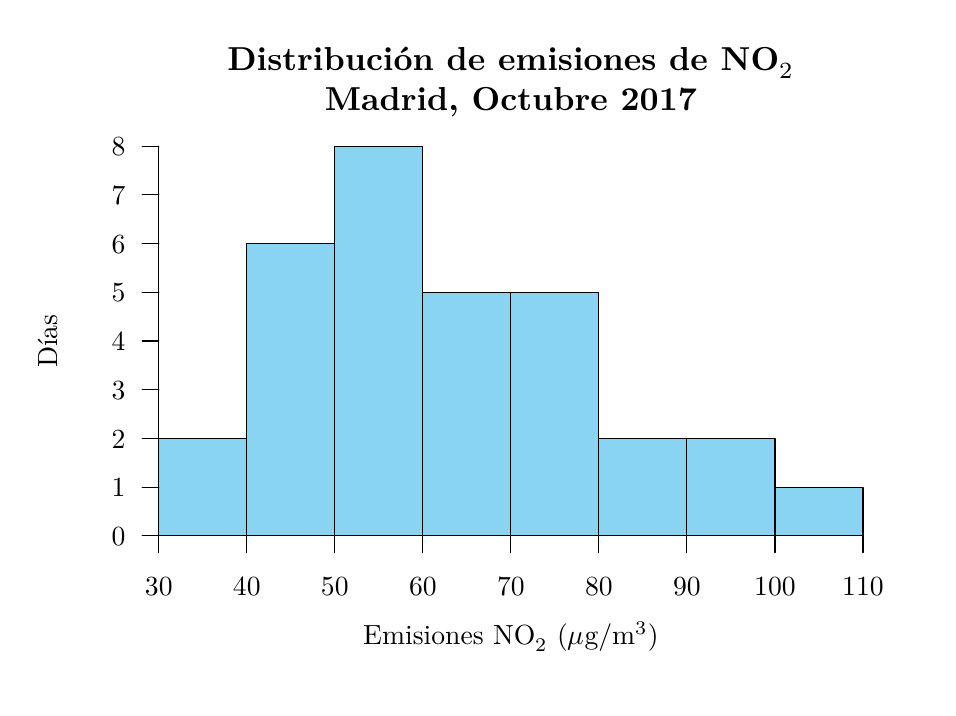
\begin{tikzpicture}[x=1pt,y=1pt]
\definecolor{fillColor}{RGB}{255,255,255}
\path[use as bounding box,fill=fillColor,fill opacity=0.00] (0,0) rectangle (325.21,238.49);
\begin{scope}
\path[clip] (  0.00,  0.00) rectangle (325.21,238.49);
\definecolor{drawColor}{RGB}{0,0,0}

\node[text=drawColor,anchor=base,inner sep=0pt, outer sep=0pt, scale=  1.20] at (174.61,222.95) {\bfseries Distribución de emisiones de NO$_2$};

\node[text=drawColor,anchor=base,inner sep=0pt, outer sep=0pt, scale=  1.20] at (174.61,208.55) {\bfseries  Madrid, Octubre 2017};

\node[text=drawColor,anchor=base,inner sep=0pt, outer sep=0pt, scale=  1.00] at (174.61, 15.60) {Emisiones NO$_2$ ($\mu$g/m$^3$)};

\node[text=drawColor,rotate= 90.00,anchor=base,inner sep=0pt, outer sep=0pt, scale=  1.00] at ( 10.80,125.25) {Días};
\end{scope}
\begin{scope}
\path[clip] ( 37.20, 49.20) rectangle (312.01,201.29);
\definecolor{drawColor}{RGB}{0,0,0}
\definecolor{fillColor}{RGB}{137,211,243}

\path[draw=drawColor,line width= 0.4pt,line join=round,line cap=round,fill=fillColor] ( 47.38, 54.83) rectangle ( 79.19, 90.04);

\path[draw=drawColor,line width= 0.4pt,line join=round,line cap=round,fill=fillColor] ( 79.19, 54.83) rectangle (110.99,160.45);

\path[draw=drawColor,line width= 0.4pt,line join=round,line cap=round,fill=fillColor] (110.99, 54.83) rectangle (142.80,195.66);

\path[draw=drawColor,line width= 0.4pt,line join=round,line cap=round,fill=fillColor] (142.80, 54.83) rectangle (174.61,142.85);

\path[draw=drawColor,line width= 0.4pt,line join=round,line cap=round,fill=fillColor] (174.61, 54.83) rectangle (206.41,142.85);

\path[draw=drawColor,line width= 0.4pt,line join=round,line cap=round,fill=fillColor] (206.41, 54.83) rectangle (238.22, 90.04);

\path[draw=drawColor,line width= 0.4pt,line join=round,line cap=round,fill=fillColor] (238.22, 54.83) rectangle (270.03, 90.04);

\path[draw=drawColor,line width= 0.4pt,line join=round,line cap=round,fill=fillColor] (270.03, 54.83) rectangle (301.84, 72.44);
\end{scope}
\begin{scope}
\path[clip] (  0.00,  0.00) rectangle (325.21,238.49);
\definecolor{drawColor}{RGB}{0,0,0}

\path[draw=drawColor,line width= 0.4pt,line join=round,line cap=round] ( 47.38, 54.83) -- (301.84, 54.83);

\path[draw=drawColor,line width= 0.4pt,line join=round,line cap=round] ( 47.38, 54.83) -- ( 47.38, 48.83);

\path[draw=drawColor,line width= 0.4pt,line join=round,line cap=round] ( 79.19, 54.83) -- ( 79.19, 48.83);

\path[draw=drawColor,line width= 0.4pt,line join=round,line cap=round] (110.99, 54.83) -- (110.99, 48.83);

\path[draw=drawColor,line width= 0.4pt,line join=round,line cap=round] (142.80, 54.83) -- (142.80, 48.83);

\path[draw=drawColor,line width= 0.4pt,line join=round,line cap=round] (174.61, 54.83) -- (174.61, 48.83);

\path[draw=drawColor,line width= 0.4pt,line join=round,line cap=round] (206.41, 54.83) -- (206.41, 48.83);

\path[draw=drawColor,line width= 0.4pt,line join=round,line cap=round] (238.22, 54.83) -- (238.22, 48.83);

\path[draw=drawColor,line width= 0.4pt,line join=round,line cap=round] (270.03, 54.83) -- (270.03, 48.83);

\path[draw=drawColor,line width= 0.4pt,line join=round,line cap=round] (301.84, 54.83) -- (301.84, 48.83);

\node[text=drawColor,anchor=base,inner sep=0pt, outer sep=0pt, scale=  1.00] at ( 47.38, 33.23) {30};

\node[text=drawColor,anchor=base,inner sep=0pt, outer sep=0pt, scale=  1.00] at ( 79.19, 33.23) {40};

\node[text=drawColor,anchor=base,inner sep=0pt, outer sep=0pt, scale=  1.00] at (110.99, 33.23) {50};

\node[text=drawColor,anchor=base,inner sep=0pt, outer sep=0pt, scale=  1.00] at (142.80, 33.23) {60};

\node[text=drawColor,anchor=base,inner sep=0pt, outer sep=0pt, scale=  1.00] at (174.61, 33.23) {70};

\node[text=drawColor,anchor=base,inner sep=0pt, outer sep=0pt, scale=  1.00] at (206.41, 33.23) {80};

\node[text=drawColor,anchor=base,inner sep=0pt, outer sep=0pt, scale=  1.00] at (238.22, 33.23) {90};

\node[text=drawColor,anchor=base,inner sep=0pt, outer sep=0pt, scale=  1.00] at (270.03, 33.23) {100};

\node[text=drawColor,anchor=base,inner sep=0pt, outer sep=0pt, scale=  1.00] at (301.84, 33.23) {110};

\path[draw=drawColor,line width= 0.4pt,line join=round,line cap=round] ( 47.38, 54.83) -- ( 47.38,195.66);

\path[draw=drawColor,line width= 0.4pt,line join=round,line cap=round] ( 47.38, 54.83) -- ( 41.38, 54.83);

\path[draw=drawColor,line width= 0.4pt,line join=round,line cap=round] ( 47.38, 72.44) -- ( 41.38, 72.44);

\path[draw=drawColor,line width= 0.4pt,line join=round,line cap=round] ( 47.38, 90.04) -- ( 41.38, 90.04);

\path[draw=drawColor,line width= 0.4pt,line join=round,line cap=round] ( 47.38,107.64) -- ( 41.38,107.64);

\path[draw=drawColor,line width= 0.4pt,line join=round,line cap=round] ( 47.38,125.25) -- ( 41.38,125.25);

\path[draw=drawColor,line width= 0.4pt,line join=round,line cap=round] ( 47.38,142.85) -- ( 41.38,142.85);

\path[draw=drawColor,line width= 0.4pt,line join=round,line cap=round] ( 47.38,160.45) -- ( 41.38,160.45);

\path[draw=drawColor,line width= 0.4pt,line join=round,line cap=round] ( 47.38,178.05) -- ( 41.38,178.05);

\path[draw=drawColor,line width= 0.4pt,line join=round,line cap=round] ( 47.38,195.66) -- ( 41.38,195.66);

\node[text=drawColor,anchor=base east,inner sep=0pt, outer sep=0pt, scale=  1.00] at ( 35.38, 51.39) {0};

\node[text=drawColor,anchor=base east,inner sep=0pt, outer sep=0pt, scale=  1.00] at ( 35.38, 68.99) {1};

\node[text=drawColor,anchor=base east,inner sep=0pt, outer sep=0pt, scale=  1.00] at ( 35.38, 86.60) {2};

\node[text=drawColor,anchor=base east,inner sep=0pt, outer sep=0pt, scale=  1.00] at ( 35.38,104.20) {3};

\node[text=drawColor,anchor=base east,inner sep=0pt, outer sep=0pt, scale=  1.00] at ( 35.38,121.80) {4};

\node[text=drawColor,anchor=base east,inner sep=0pt, outer sep=0pt, scale=  1.00] at ( 35.38,139.41) {5};

\node[text=drawColor,anchor=base east,inner sep=0pt, outer sep=0pt, scale=  1.00] at ( 35.38,157.01) {6};

\node[text=drawColor,anchor=base east,inner sep=0pt, outer sep=0pt, scale=  1.00] at ( 35.38,174.61) {7};

\node[text=drawColor,anchor=base east,inner sep=0pt, outer sep=0pt, scale=  1.00] at ( 35.38,192.21) {8};
\end{scope}
\end{tikzpicture}
}
	\end{center}
\end{frame}


%----------------------------------------------------------------------SLIDE----
\begin{frame}[c]
	\large
	Se pide: 
	
	\begin{enumerate}
		\item La normativa europea sobre calidad del aire establece que el valor medio mensual no debe exceder de 40 $\mu$g/m$^3$. ¿Se ha cumplido la norma en el mes de Octubre? 
		¿Es este un valor representativo de las mediciones tomadas en octubre?
		\item El Ayuntamiento de Madrid ha decidido que se establecerán restricciones de velocidad en los accesos los días en los que se superen los 72 $\mu$g/m$^3$ y que además de estas restricciones se establecerán también restricciones al aparcamiento los días que se superen los 92 $\mu$g/m$^3$.
		¿Qué porcentaje de días de octubre se establecieron solo restricciones de velocidad en los accesos?
		\item De acuerdo con esta muestra de datos tomada durante el mes de octubre, ¿puede establecerse por la forma de la distribución de la muestra que la distribución de las emisiones en toda la ciudad sigue una distribución normal?
	\end{enumerate}
\end{frame}


%----------------------------------------------------------------------SLIDE----
\begin{frame}[c]
	\large
	\begin{enumerate}
		\setcounter{enumi}{3}
		\item Además del nivel de NO$_2$, el Ayuntamiento también controla los niveles de SO$_2$, y se sabe que el nivel medio de esta sustancia durante el mes de octubre fue de $2.85$ $\mu$g/m$^3$ con una desviación típica de $0.42$ $\mu$g/m$^3$. 
		Si un día hubo un nivel de NO$_2$ de 46 y un nivel de SO$_2$ de $2.24$, ¿cuál de las dos sustancias tenía niveles más altos en referencia a sus mediciones?
		\item Si el índice de calidad del aire (ICA) puede estimarse multiplicando el nivel de NO$_2$ por $0.90$ y sumándole una cantidad fija de 30. 
		¿Cuál fue el índice medio de la calidad del aire en Madrid el mes de octubre? 
		¿Es un valor más o menos representativo que el nivel de emisiones medio de NO$_2$?
		\item ¿Existen días atípicos en las emisiones de NO$_2$ del mes de octubre? Justificar la respuesta.
	\end{enumerate}
	Utilizar las siguientes sumas para los cálculos: $\sum x_i=1945$ $\mu$g/m$^3$, $\sum x_i^2=131575$ ($\mu$g/m$^3$)$^2$, $\sum (x_i-\bar x)^3=93995.838$ ($\mu$g/m$^3$)$^3$ y $\sum (x_i-\bar x)^4=7766271.021$ ($\mu$g/m$^3$)$^4$.
\end{frame}


%----------------------------------------------------------------------SLIDE----
\begin{frame}
	\begin{columns}
		\begin{column}[T]{0.55\textwidth}
			\begin{enumerate}
				\item La normativa europea sobre calidad del aire establece que el valor medio mensual no debe exceder de 40 $\mu$g/m$^3$. ¿Se ha cumplido la norma en el mes de Octubre? 
				¿Es este un valor representativo de las mediciones tomadas en octubre?		
			\end{enumerate}
		\end{column}
		\begin{column}[T]{0.45\textwidth}
			\begin{datos}
				$X\equiv$ Emisiones de NO$_2$\\
				$\sum x_i=1945$ $\mu$g/m$^3$\\
				$\sum x_i^2=131575$ ($\mu$g/m$^3$)$^2$\\
				$\sum (x_i-\bar x)^3=93995.838$ ($\mu$g/m$^3$)$^3$\\
				$\sum (x_i-\bar x)^4=7766271.021$ ($\mu$g/m$^3$)$^4$
			\end{datos}
		\end{column}
	\end{columns}
\end{frame}


%----------------------------------------------------------------------SLIDE----
\begin{frame}
	\begin{columns}
		\begin{column}[T]{0.55\textwidth}
			\begin{enumerate}
				\item[2.] El Ayuntamiento de Madrid ha decidido que se establecerán restricciones de velocidad en los accesos los días en los que se superen los 72 $\mu$g/m$^3$ y que además de estas restricciones se establecerán también restricciones al aparcamiento los días que se superen los 92 $\mu$g/m$^3$.
		¿Qué porcentaje de días de octubre se establecieron solo restricciones de velocidad en los accesos?
			\end{enumerate}
		\end{column}
		\begin{column}[T]{0.45\textwidth}
			\begin{datos}
				\resizebox{\textwidth}{!}{% Created by tikzDevice version 0.10.1 on 2017-11-26 21:00:39
% !TEX encoding = UTF-8 Unicode
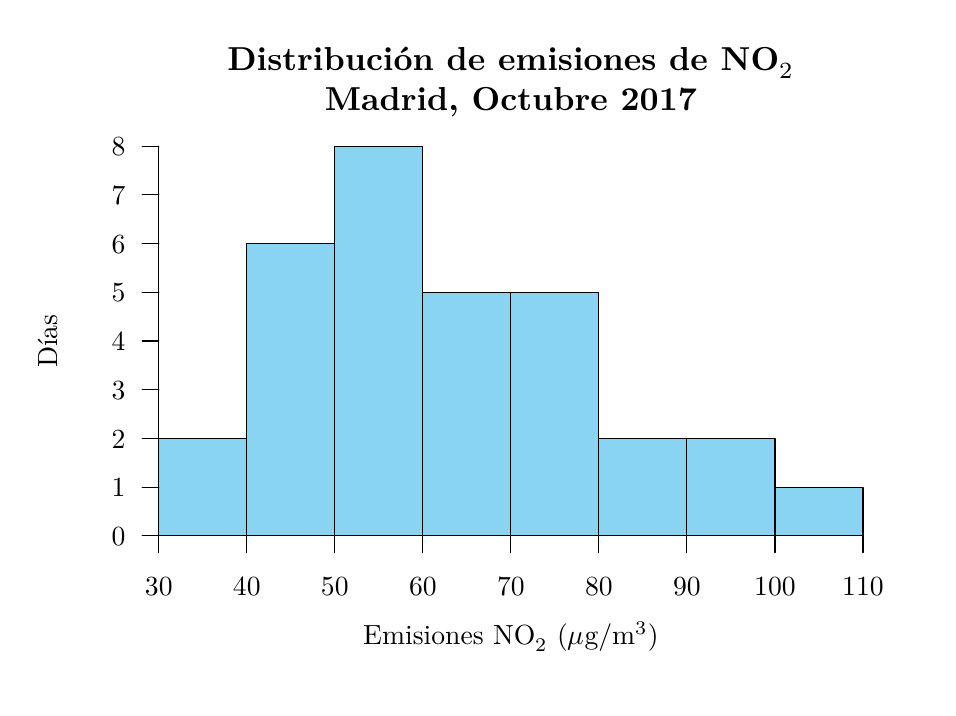
\begin{tikzpicture}[x=1pt,y=1pt]
\definecolor{fillColor}{RGB}{255,255,255}
\path[use as bounding box,fill=fillColor,fill opacity=0.00] (0,0) rectangle (325.21,238.49);
\begin{scope}
\path[clip] (  0.00,  0.00) rectangle (325.21,238.49);
\definecolor{drawColor}{RGB}{0,0,0}

\node[text=drawColor,anchor=base,inner sep=0pt, outer sep=0pt, scale=  1.20] at (174.61,222.95) {\bfseries Distribución de emisiones de NO$_2$};

\node[text=drawColor,anchor=base,inner sep=0pt, outer sep=0pt, scale=  1.20] at (174.61,208.55) {\bfseries  Madrid, Octubre 2017};

\node[text=drawColor,anchor=base,inner sep=0pt, outer sep=0pt, scale=  1.00] at (174.61, 15.60) {Emisiones NO$_2$ ($\mu$g/m$^3$)};

\node[text=drawColor,rotate= 90.00,anchor=base,inner sep=0pt, outer sep=0pt, scale=  1.00] at ( 10.80,125.25) {Días};
\end{scope}
\begin{scope}
\path[clip] ( 37.20, 49.20) rectangle (312.01,201.29);
\definecolor{drawColor}{RGB}{0,0,0}
\definecolor{fillColor}{RGB}{137,211,243}

\path[draw=drawColor,line width= 0.4pt,line join=round,line cap=round,fill=fillColor] ( 47.38, 54.83) rectangle ( 79.19, 90.04);

\path[draw=drawColor,line width= 0.4pt,line join=round,line cap=round,fill=fillColor] ( 79.19, 54.83) rectangle (110.99,160.45);

\path[draw=drawColor,line width= 0.4pt,line join=round,line cap=round,fill=fillColor] (110.99, 54.83) rectangle (142.80,195.66);

\path[draw=drawColor,line width= 0.4pt,line join=round,line cap=round,fill=fillColor] (142.80, 54.83) rectangle (174.61,142.85);

\path[draw=drawColor,line width= 0.4pt,line join=round,line cap=round,fill=fillColor] (174.61, 54.83) rectangle (206.41,142.85);

\path[draw=drawColor,line width= 0.4pt,line join=round,line cap=round,fill=fillColor] (206.41, 54.83) rectangle (238.22, 90.04);

\path[draw=drawColor,line width= 0.4pt,line join=round,line cap=round,fill=fillColor] (238.22, 54.83) rectangle (270.03, 90.04);

\path[draw=drawColor,line width= 0.4pt,line join=round,line cap=round,fill=fillColor] (270.03, 54.83) rectangle (301.84, 72.44);
\end{scope}
\begin{scope}
\path[clip] (  0.00,  0.00) rectangle (325.21,238.49);
\definecolor{drawColor}{RGB}{0,0,0}

\path[draw=drawColor,line width= 0.4pt,line join=round,line cap=round] ( 47.38, 54.83) -- (301.84, 54.83);

\path[draw=drawColor,line width= 0.4pt,line join=round,line cap=round] ( 47.38, 54.83) -- ( 47.38, 48.83);

\path[draw=drawColor,line width= 0.4pt,line join=round,line cap=round] ( 79.19, 54.83) -- ( 79.19, 48.83);

\path[draw=drawColor,line width= 0.4pt,line join=round,line cap=round] (110.99, 54.83) -- (110.99, 48.83);

\path[draw=drawColor,line width= 0.4pt,line join=round,line cap=round] (142.80, 54.83) -- (142.80, 48.83);

\path[draw=drawColor,line width= 0.4pt,line join=round,line cap=round] (174.61, 54.83) -- (174.61, 48.83);

\path[draw=drawColor,line width= 0.4pt,line join=round,line cap=round] (206.41, 54.83) -- (206.41, 48.83);

\path[draw=drawColor,line width= 0.4pt,line join=round,line cap=round] (238.22, 54.83) -- (238.22, 48.83);

\path[draw=drawColor,line width= 0.4pt,line join=round,line cap=round] (270.03, 54.83) -- (270.03, 48.83);

\path[draw=drawColor,line width= 0.4pt,line join=round,line cap=round] (301.84, 54.83) -- (301.84, 48.83);

\node[text=drawColor,anchor=base,inner sep=0pt, outer sep=0pt, scale=  1.00] at ( 47.38, 33.23) {30};

\node[text=drawColor,anchor=base,inner sep=0pt, outer sep=0pt, scale=  1.00] at ( 79.19, 33.23) {40};

\node[text=drawColor,anchor=base,inner sep=0pt, outer sep=0pt, scale=  1.00] at (110.99, 33.23) {50};

\node[text=drawColor,anchor=base,inner sep=0pt, outer sep=0pt, scale=  1.00] at (142.80, 33.23) {60};

\node[text=drawColor,anchor=base,inner sep=0pt, outer sep=0pt, scale=  1.00] at (174.61, 33.23) {70};

\node[text=drawColor,anchor=base,inner sep=0pt, outer sep=0pt, scale=  1.00] at (206.41, 33.23) {80};

\node[text=drawColor,anchor=base,inner sep=0pt, outer sep=0pt, scale=  1.00] at (238.22, 33.23) {90};

\node[text=drawColor,anchor=base,inner sep=0pt, outer sep=0pt, scale=  1.00] at (270.03, 33.23) {100};

\node[text=drawColor,anchor=base,inner sep=0pt, outer sep=0pt, scale=  1.00] at (301.84, 33.23) {110};

\path[draw=drawColor,line width= 0.4pt,line join=round,line cap=round] ( 47.38, 54.83) -- ( 47.38,195.66);

\path[draw=drawColor,line width= 0.4pt,line join=round,line cap=round] ( 47.38, 54.83) -- ( 41.38, 54.83);

\path[draw=drawColor,line width= 0.4pt,line join=round,line cap=round] ( 47.38, 72.44) -- ( 41.38, 72.44);

\path[draw=drawColor,line width= 0.4pt,line join=round,line cap=round] ( 47.38, 90.04) -- ( 41.38, 90.04);

\path[draw=drawColor,line width= 0.4pt,line join=round,line cap=round] ( 47.38,107.64) -- ( 41.38,107.64);

\path[draw=drawColor,line width= 0.4pt,line join=round,line cap=round] ( 47.38,125.25) -- ( 41.38,125.25);

\path[draw=drawColor,line width= 0.4pt,line join=round,line cap=round] ( 47.38,142.85) -- ( 41.38,142.85);

\path[draw=drawColor,line width= 0.4pt,line join=round,line cap=round] ( 47.38,160.45) -- ( 41.38,160.45);

\path[draw=drawColor,line width= 0.4pt,line join=round,line cap=round] ( 47.38,178.05) -- ( 41.38,178.05);

\path[draw=drawColor,line width= 0.4pt,line join=round,line cap=round] ( 47.38,195.66) -- ( 41.38,195.66);

\node[text=drawColor,anchor=base east,inner sep=0pt, outer sep=0pt, scale=  1.00] at ( 35.38, 51.39) {0};

\node[text=drawColor,anchor=base east,inner sep=0pt, outer sep=0pt, scale=  1.00] at ( 35.38, 68.99) {1};

\node[text=drawColor,anchor=base east,inner sep=0pt, outer sep=0pt, scale=  1.00] at ( 35.38, 86.60) {2};

\node[text=drawColor,anchor=base east,inner sep=0pt, outer sep=0pt, scale=  1.00] at ( 35.38,104.20) {3};

\node[text=drawColor,anchor=base east,inner sep=0pt, outer sep=0pt, scale=  1.00] at ( 35.38,121.80) {4};

\node[text=drawColor,anchor=base east,inner sep=0pt, outer sep=0pt, scale=  1.00] at ( 35.38,139.41) {5};

\node[text=drawColor,anchor=base east,inner sep=0pt, outer sep=0pt, scale=  1.00] at ( 35.38,157.01) {6};

\node[text=drawColor,anchor=base east,inner sep=0pt, outer sep=0pt, scale=  1.00] at ( 35.38,174.61) {7};

\node[text=drawColor,anchor=base east,inner sep=0pt, outer sep=0pt, scale=  1.00] at ( 35.38,192.21) {8};
\end{scope}
\end{tikzpicture}
}
			\end{datos}
		\end{column}
	\end{columns}
\end{frame}


%----------------------------------------------------------------------SLIDE----
\begin{frame}
	\begin{columns}
		\begin{column}[T]{0.7\textwidth}
			\begin{enumerate}
				\item[2.] El Ayuntamiento de Madrid ha decidido que se establecerán restricciones de velocidad en los accesos los días en los que se superen los 72 $\mu$g/m$^3$ y que además de estas restricciones se establecerán también restricciones al aparcamiento los días que se superen los 92 $\mu$g/m$^3$.
				¿Qué porcentaje de días de octubre se establecieron solo restricciones de velocidad en los accesos?
			\end{enumerate}
		\end{column}
		\begin{column}[T]{0.3\textwidth}
			\begin{datos}
			$X\equiv$ Emisiones de NO$_2$\\
			\[
				\begin{array}{cc}
					X & F_i\\
					\midrule
					30 - 40 & 0.0645\\
    			40 - 50 & 0.2581\\
    			50 - 60 & 0.5161\\
    			60 - 70 & 0.6774\\
    			70 - 80 & 0.8387\\
    			80 - 90 & 0.9032\\
    			90 - 100 & 0.9677\\
    			100 - 110 & 1.0000\\
					\bottomrule
				\end{array}
			\]
			\end{datos}
		\end{column}
	\end{columns}
\end{frame}


%----------------------------------------------------------------------SLIDE----
\begin{frame}
	\begin{columns}
		\begin{column}[T]{0.7\textwidth}
			\begin{enumerate}
				\item[2.] El Ayuntamiento de Madrid ha decidido que se establecerán restricciones de velocidad en los accesos los días en los que se superen los 72 $\mu$g/m$^3$ y que además de estas restricciones se establecerán también restricciones al aparcamiento los días que se superen los 92 $\mu$g/m$^3$.
				¿Qué porcentaje de días de octubre se establecieron solo restricciones de velocidad en los accesos?
			\end{enumerate}
		\end{column}
		\begin{column}[T]{0.3\textwidth}
			\begin{datos}
			$X\equiv$ Emisiones de NO$_2$\\
			\[
				\begin{array}{cc}
					X & F_i\\
					\midrule
					30 - 40 & 0.0645\\
    			40 - 50 & 0.2581\\
    			50 - 60 & 0.5161\\
    			60 - 70 & 0.6774\\
    			70 - 80 & 0.8387\\
    			80 - 90 & 0.9032\\
    			90 - 100 & 0.9677\\
    			100 - 110 & 1.0000\\
					\bottomrule
				\end{array}
			\]
			\end{datos}
		\end{column}
	\end{columns}
\end{frame}


%----------------------------------------------------------------------SLIDE----
\begin{frame}
	\begin{columns}
		\begin{column}[T]{0.7\textwidth}
			\begin{enumerate}
				\item[2.] El Ayuntamiento de Madrid ha decidido que se establecerán restricciones de velocidad en los accesos los días en los que se superen los 72 $\mu$g/m$^3$ y que además de estas restricciones se establecerán también restricciones al aparcamiento los días que se superen los 92 $\mu$g/m$^3$.
				¿Qué porcentaje de días de octubre se establecieron solo restricciones de velocidad en los accesos?
			\end{enumerate}
		\end{column}
		\begin{column}[T]{0.3\textwidth}
			\begin{datos}
			$X\equiv$ Emisiones de NO$_2$\\
			\[
				\begin{array}{cc}
					X & F_i\\
					\midrule
					30 - 40 & 0.0645\\
    			40 - 50 & 0.2581\\
    			50 - 60 & 0.5161\\
    			60 - 70 & 0.6774\\
    			70 - 80 & 0.8387\\
    			80 - 90 & 0.9032\\
    			90 - 100 & 0.9677\\
    			100 - 110 & 1.0000\\
					\bottomrule
				\end{array}
			\]
			F(92)=0.9161
			\end{datos}
		\end{column}
	\end{columns}
\end{frame}


%----------------------------------------------------------------------SLIDE----
\begin{frame}
	\begin{columns}
		\begin{column}[T]{0.55\textwidth}
			\begin{enumerate}
				\item[3.] De acuerdo con esta muestra de datos tomada durante el mes de octubre, ¿puede establecerse por la forma de la distribución de la muestra que la distribución de las emisiones en toda la ciudad sigue una distribución normal?
			\end{enumerate}
		\end{column}
		\begin{column}[T]{0.45\textwidth}
			\begin{datos}
				$X\equiv$ Emisiones de NO$_2$\\
				$\sum (x_i-\bar x)^3=93995.838$ ($\mu$g/m$^3$)$^3$\\
				$\sum (x_i-\bar x)^4=7766271.021$ ($\mu$g/m$^3$)$^4$\\
				$\bar x = 62.7419$ $\mu$g/m$^3$\\
				$s_x=17.5444$ $\mu$g/m$^3$
			\end{datos}
		\end{column}
	\end{columns}
\end{frame}


%----------------------------------------------------------------------SLIDE----
\begin{frame}
	\begin{columns}
		\begin{column}[T]{0.65\textwidth}
			\begin{enumerate}
				\item[4.] Además del nivel de NO$_2$, el Ayuntamiento también controla los niveles de SO$_2$, y se sabe que el nivel medio de esta sustancia durante el mes de octubre fue de $2.85$ $\mu$g/m$^3$ con una desviación típica de $0.42$ $\mu$g/m$^3$. 
				Si un día hubo un nivel de NO$_2$ de 46 y un nivel de SO$_2$ de $2.24$, ¿cuál de las dos sustancias tenía niveles más altos en referencia a sus mediciones?
			\end{enumerate}
		\end{column}
		\begin{column}[T]{0.35\textwidth}
			\begin{datos}
				$X\equiv$ Emisiones de NO$_2$\\
				$Y\equiv$ Emisiones de SO$_2$\\
				$\bar x = 62.7419$ $\mu$g/m$^3$\\
				$s_x=17.5444$ $\mu$g/m$^3$\\
				$\bar y=2.85$ $\mu$g/m$^3$\\
				$s_y=0.42$ $\mu$g/m$^3$
			\end{datos}
		\end{column}
	\end{columns}
\end{frame}


%----------------------------------------------------------------------SLIDE----
\begin{frame}
	\begin{columns}
		\begin{column}[T]{0.65\textwidth}
			\begin{enumerate}
				\item[5.] Si el índice de calidad del aire (ICA) puede estimarse multiplicando el nivel de NO$_2$ por $0.90$ y sumándole una cantidad fija de 30. 
		¿Cuál fue el índice medio de la calidad del aire en Madrid el mes de octubre? 
		¿Es un valor más o menos representativo que el nivel de emisiones medio de NO$_2$?
			\end{enumerate}
		\end{column}
		\begin{column}[T]{0.35\textwidth}
			\begin{datos}
				$X\equiv$ Emisiones de NO$_2$\\
				$\bar x = 62.7419$ $\mu$g/m$^3$\\
				$s_x=17.5444$ $\mu$g/m$^3$\\
			\end{datos}
		\end{column}
	\end{columns}
\end{frame}


%----------------------------------------------------------------------SLIDE----
\begin{frame}
	\begin{columns}
		\begin{column}[T]{0.7\textwidth}
			\begin{enumerate}
				\item[6.] ¿Existen días atípicos en las emisiones de NO$_2$ del mes de octubre? Justificar la respuesta.
			\end{enumerate}
		\end{column}
		\begin{column}[T]{0.3\textwidth}
			\begin{datos}
			$X\equiv$ Emisiones de NO$_2$\\
			\[
				\begin{array}{cc}
					X & F_i\\
					\midrule
					30 - 40 & 0.0645\\
    			40 - 50 & 0.2581\\
    			50 - 60 & 0.5161\\
    			60 - 70 & 0.6774\\
    			70 - 80 & 0.8387\\
    			80 - 90 & 0.9032\\
    			90 - 100 & 0.9677\\
    			100 - 110 & 1.0000\\
					\bottomrule
				\end{array}
			\]
			\end{datos}
		\end{column}
	\end{columns}
\end{frame}

\end{document}
